\begin{figure}[h!]
  \centering
  \caption{\label{fig:metalinter_report}A MegaLinter report that was automatically attached as a comment to a pull request.}
  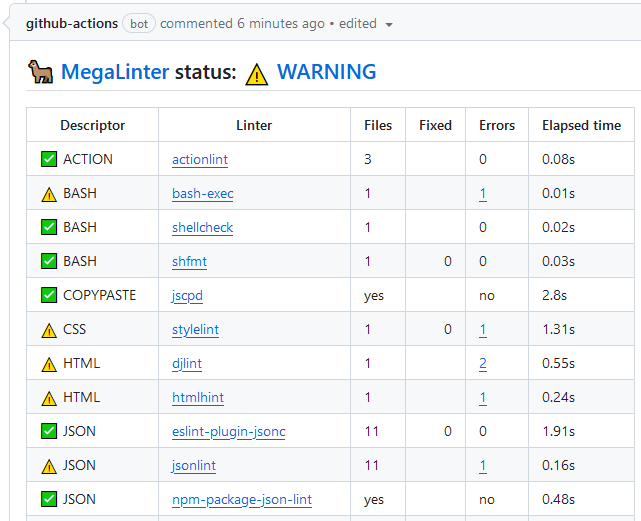
\includegraphics[width=\textwidth]{figures/megalinter_report.png}
\end{figure}

\begin{figure}
  \centering
  \caption{\label{fig:similarity_flamegraph}Flame graph for the similarity endpoint. Most time is spent in matrix maths functions}
  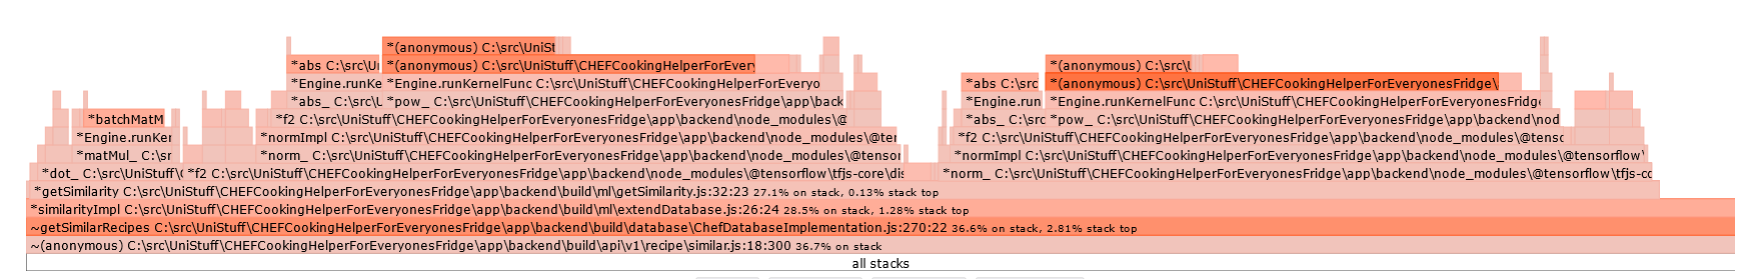
\includegraphics[angle=90,height=0.9\textheight]{figures/similarity_flamegraph.png}
\end{figure}

\begin{figure}
  \centering
  \caption{\label{fig:test_report}A test report showing that all tests passed.}
  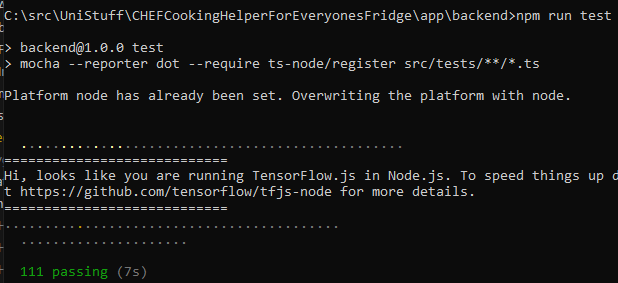
\includegraphics[width=0.9\textwidth]{figures/test_report.png}
\end{figure}

\begin{figure}
  \centering
  \caption{\label{fig:coverage_report}A coverage report showing which lines were and were not executed during test cases.}
  \todo{Update once coverage is higher}
  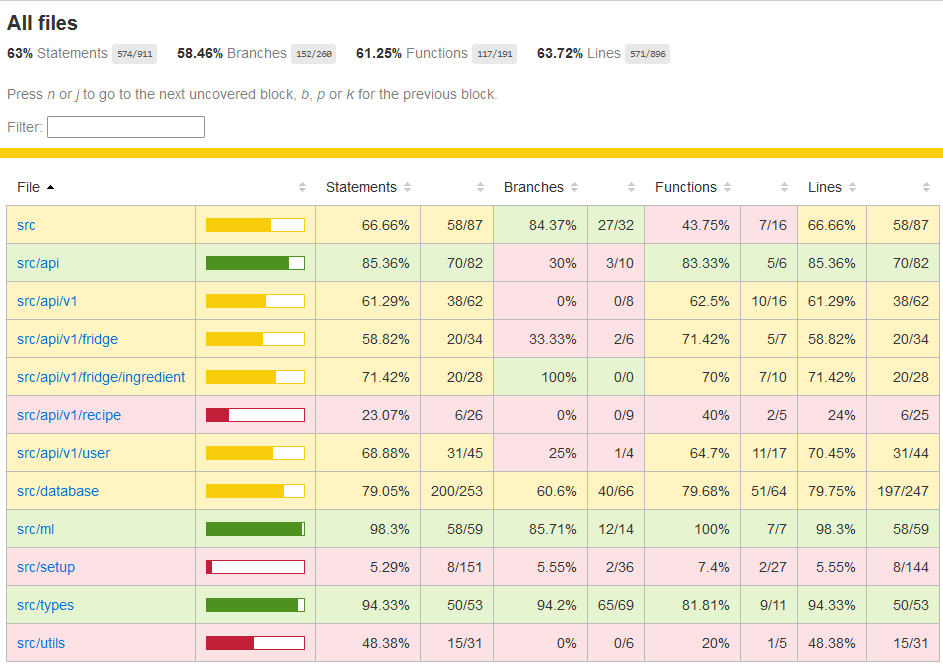
\includegraphics[width=0.9\textwidth]{figures/coverage_report.png}
\end{figure}

\cleartoleftpage\begin{figure}
  \centering
  \caption{\label{fig:search_query}The query used to search recipes}
  \begin{verbatim}
SELECT
recipe.name, recipe.id,
-- COUNT excludes NULLs.
COUNT(
  CASE
    -- If fridgeId is null, then we can't
    -- create a meaningful missing count
    WHEN :fridgeId IS NULL THEN NULL

    -- Check if we have any of the ingredients
    WHEN fridge_ingredient.amount IS NULL THEN 1

    -- Optionally check if we have enough of the ingredients
    WHEN
      :checkAmount AND
      fridge_ingredient.amount < recipe_ingredient.amount
      THEN 1
  END) as missing_count,
CASE WHEN :search IS NULL
  THEN NULL
  ELSE ml_similarity(embedding.embedding, :search)
END AS similarity
FROM recipe
JOIN embedding ON embedding.sentence = recipe.name
LEFT JOIN recipe_ingredient ON
  recipe_ingredient.recipe_id = recipe.id
LEFT JOIN fridge_ingredient ON
  fridge_ingredient.ingredient_id = recipe_ingredient.ingredient_id
    AND
  fridge_ingredient.fridge_id = :fridgeId
JOIN ingredient ON
  ingredient.id = recipe_ingredient.ingredient_id AND
  NOT ingredient.assumeUnlimited
LEFT JOIN ingredient_tag ON
  ingredient_tag.ingredient_id = ingredient.id
WHERE (
recipe.meal_type_id = (
  SELECT id FROM meal_type WHERE name = :mealType
) OR :mealType IS NULL
) AND (similarity >= :minSimilarity OR :search IS NULL)
GROUP BY recipe.id
  \end{verbatim}
\end{figure}

\begin{figure}\ContinuedFloat{}
  \begin{verbatim}
HAVING
(missing_count <= :maxMissingIngredients OR :fridgeId IS NULL)
-- SUM(CASE WHEN ... THEN 1 ELSE 0 END) = 0
-- checks for CASE WHEN returning false for all rows
-- No banned tags
AND (SUM(CASE WHEN
  ingredient_tag.tag_id IN
    (SELECT tag_id FROM ${bannedTagsTable})
THEN 1 ELSE 0 END) = 0)
-- No banned ingredients
AND (SUM(CASE WHEN
  recipe_ingredient.ingredient_id IN
    (SELECT ingredient_id FROM ${bannedIngredsTable})
THEN 1 ELSE 0 END) = 0)
ORDER BY missing_count ASC, similarity DESC
LIMIT :limit
  \end{verbatim}
\end{figure}
